\section{Worksheet 1}
The deafault rendering of the framework can be seen in figure \ref{fig:preview}.
\begin{figure}[H]
	\centering
	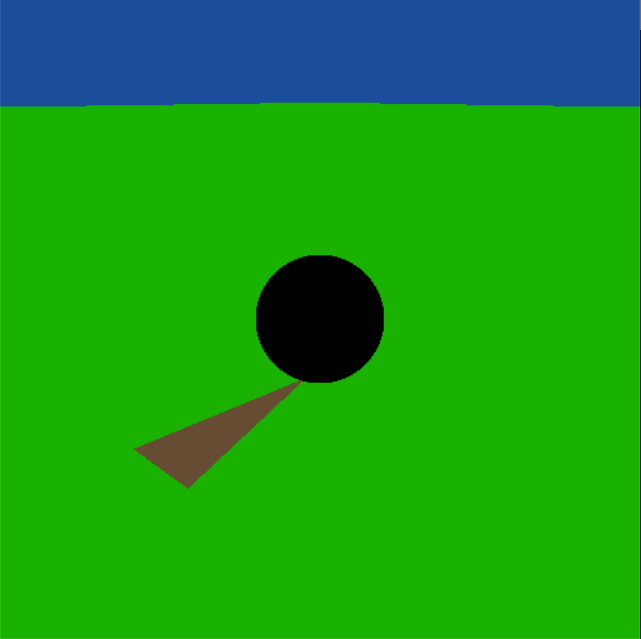
\includegraphics[scale=\imagescale]{images/worksheet_1/preview}
	\caption{Default rendering}
	\label{fig:preview}
\end{figure}
The first thing we do is implementing the render function in the RenderEngine class which loops over all pixels. For now the compute\_pixel function returns only red pixels.
\begin{lstlisting}
void RenderEngine::render()
{
	cout << "Raytracing";
	Timer timer;
	timer.start();
	
	int x_res = static_cast<int>(res.x);
	int y_res = static_cast<int>(res.y);
	#pragma omp parallel for private(randomizer)
	for(int y = 0; y < y_res ; ++y)
	{
		for (int x = 0; x < x_res; ++x)
		{
			image[x+y*y_res] = tracer.compute_pixel(x, y);
		}
		if(((y + 1) % 50) == 0) 
		cerr << ".";
	}
	
	timer.stop();
	cout << " - " << timer.get_time() << " secs " << endl;
	init_texture();
	done = true;
}
\end{lstlisting}
Then we proceed to implementing the set, get\_ray\_dir and get\_ray direction that we can find in the Camera class.
\begin{lstlisting}
void Camera::set(const float3& eye_point, const float3& view_point, const float3& up_vector, float camera_constant)
{
	eye = eye_point;
	lookat = view_point;
	up = up_vector;
	cam_const = camera_constant;
	
	ip_normal = normalize(lookat - eye) ;
	ip_xaxis = normalize(cross(ip_normal, up));
	ip_yaxis = cross(ip_xaxis, ip_normal);
	
	float fov_rad = 2 * atan(1/(2 * cam_const));
	fov = fov_rad * 180 * M_1_PIf;
}

float3 Camera::get_ray_dir(const float2& coords) const{
	float3 q = ip_xaxis * coords.x + ip_yaxis * coords.y + ip_normal * cam_const;
	return normalize(q);
}

Ray Camera::get_ray(const float2& coords) const{
	float3 dir = get_ray_dir(coords);
	Ray r = Ray(eye, dir, 0,0, RT_DEFAULT_MAX);
	return r; 
}
\end{lstlisting}
Now we implement the closest\_hit function of the Accelerator class which will allow us to check the closest primitive to which our ray intersects to.
\begin{lstlisting}
bool Accelerator::closest_hit(optix::Ray& r, HitInfo& hit) const
{
	closest_plane(r, hit);
	
	for (unsigned int i = 0; i < primitives.size(); ++i)
		if (primitives[i]->geometry->intersect(r, hit, 0))
			r.tmax = hit.dist;
	return hit.has_hit;
}
\end{lstlisting}
Now we can implement the compute\_pixel function that we used before in the render function of RenderEngine.
\begin{lstlisting}
	float3 RayCaster::compute_pixel(unsigned int x, unsigned int y) const
	{
		Camera* camera = scene->get_camera();
		float2 coords = make_float2(lower_left.x + win_to_ip.x * x, lower_left.y + win_to_ip.y * y);
		float3 color = make_float3(0.0f);
		
		
		Ray ray = camera->get_ray(coords);
		
		HitInfo hit = HitInfo();
		bool has_hit = scene->closest_hit(ray, hit);
		if (has_hit) {
			color=color+ get_shader(hit)->shade(ray, hit);
		}
		else {
			color = color + get_background(ray.direction);
		}
		
		return color;
	}
\end{lstlisting}
After the previous step we should obtain a fully blue image, as the colour of the background, since the intersect function of our primitive objects isn't implemented yet. In our scene we have a sphere, a plane and a triangle. 
\begin{lstlisting}
bool Sphere::intersect(const Ray& r, HitInfo& hit, unsigned int prim_idx) const
{
	float b_half = dot((r.origin - center), r.direction);
	float c = dot((r.origin - center), (r.origin - center)) - (radius * radius);
	float t1 = -b_half - sqrt((b_half * b_half) - c);
	float t2 = -b_half + sqrt((b_half * b_half) - c);
	
	float min_t;
	if (t1 < t2) {
		min_t = t1;;
	}
	else {
		min_t = t2;
	}
	
	bool intersected = ((b_half * b_half) - c) > 0;
	bool has_hit=  intersected && min_t>r.tmin && min_t<r.tmax;
	float3 normal = normalize(hit.position-center);
	if (has_hit) {
		hit.has_hit = true;
		hit.dist = min_t;
		hit.material = &material;
		hit.geometric_normal = normal;
		hit.shading_normal = normal;
		hit.position = r.origin + r.direction * hit.dist;
	}
	return has_hit;
}

bool intersect_triangle(const Ray& ray, const float3& v0, const float3& v1, 
const float3& v2, float3& n,float& t,float& v,float& w)
{
	float3 e0 = v1 - v0;
	float3 e1 = v0 - v2;
	n = cross(e0, e1);
	float d = dot(-v0, n);
	t = dot((v0 - ray.origin), n) / dot(ray.direction, n);
	
	v = dot(cross((v0 - ray.origin), ray.direction), e1)/dot(ray.direction,n);
	w =  dot(cross((v0 - ray.origin), ray.direction), e0) / dot(ray.direction, n);
	float u = 1 - v - w;
	bool on_plane = dot(ray.direction, n) != 0;
	bool inside_triangle = v >= 0 && w >= 0 && v + w <= 1;
	bool has_hit = on_plane && inside_triangle && t > ray.tmin && t < ray.tmax;
	return has_hit;
}


bool Triangle::intersect(const Ray& r, HitInfo& hit, unsigned int prim_idx) const
{
	float3 n;
	float t;
	float v;
	float w;
	bool has_hit=::intersect_triangle(r,v0,v1,v2,n,t,v,w);
	
	if (has_hit) {
		hit.has_hit = true;
		hit.dist = t;
		hit.geometric_normal = -normalize(n);
		hit.shading_normal = -normalize(n);
		hit.material = &material;
		hit.position = r.origin + r.direction * hit.dist;
	}
	return has_hit;
}

bool Plane::intersect(const Ray& r, HitInfo& hit, unsigned int prim_idx) const
{
	float t1 = -(dot(r.origin, onb.m_normal) + d) / dot(r.direction, onb.m_normal);
	bool intersect = dot(r.direction, onb.m_normal) != 0;
	bool has_hit =  intersect && t1 > r.tmin && t1 < r.tmax;
	if (has_hit){
		hit.has_hit = true;
		hit.dist = t1;
		hit.position = r.origin + (r.direction * t1);
		hit.geometric_normal = normalize(onb.m_normal);
		hit.shading_normal = normalize(onb.m_normal);
		hit.material = &material;
	}
	return has_hit;
}
\end{lstlisting}
Now that we have implemented all of the core methods of our ray tracing framework we can see a render of the image which is really similar to default one like the one that can be seen in figure \ref{fig:default_shading}.
\begin{figure}[H]
	\centering
	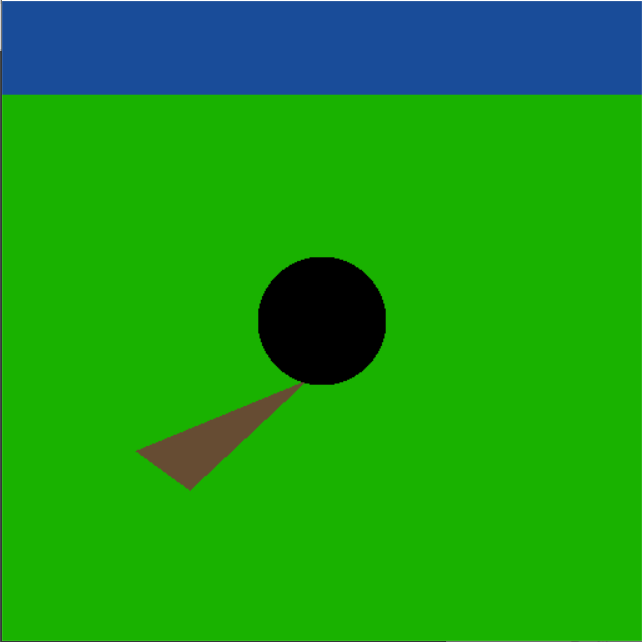
\includegraphics[scale=\imagescale]{images/worksheet_1/default_shading}
	\caption{RayTracing with default shading}
	\label{fig:default_shading}
\end{figure}
The results is almost identical to the one that we can see in the preview, the only differnece is that some of the aliasing artifacts present at the end of the plane have disappeared.\\
Now we implement lambertian shading by implementing the function PointLight::sample and the function Lambertian::shade. 
\begin{lstlisting}
bool PointLight::sample(const float3& pos, float3& dir, float3& L) const
{	
	dir = light_pos - pos;
	L = intensity / sqrt(pow(dir.x, 2) + pow(dir.y, 2) + pow(dir.z, 2));
	return false;
}

float3 Lambertian::shade(const Ray& r, HitInfo& hit, bool emit) const
{
	float3 rho_d = get_diffuse(hit);
	float3 result = make_float3(0.0f);

	for (int i = 0; i < lights.size();i++) {
		float3 dir;
		float3 L;
		
		bool shade=lights[i]->sample(hit.position, dir, L);
		if (dot(dir, hit.shading_normal) > 0) {
			result = result + (rho_d / M_PIf) * L * (dot(dir, hit.shading_normal));
		}
	}
	return result + Emission::shade(r, hit, emit);
}
\end{lstlisting}
\begin{figure}[H]
	\centering
	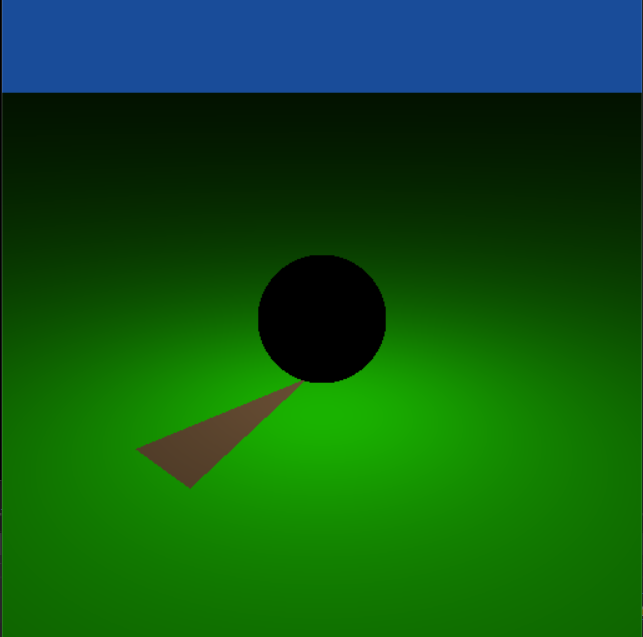
\includegraphics[scale=\imagescale]{images/worksheet_1/shading_of_diffuse_objects}
	\caption{}
	\label{fig:diffuse_shading}
\end{figure}